% !TeX spellcheck = cs_CZ

% xelatex -enable-write18 -shell-escape mai_fig021.tex

\documentclass{standalone}
\usepackage{tikz}
  \usetikzlibrary{intersections, calc, positioning}
  \usetikzlibrary{decorations.pathmorphing, decorations.pathreplacing} 
  \usetikzlibrary{matrix, arrows}
  \usetikzlibrary{chains}
  \usetikzlibrary{quotes, shapes}
\usepackage{pgfplots}
  \pgfplotsset{compat=newest}
  
\begin{document}
  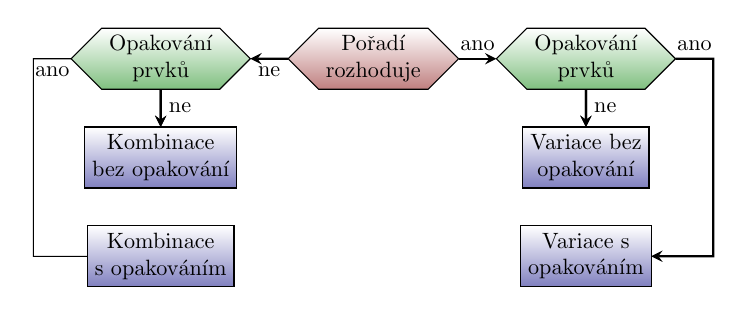
\begin{tikzpicture}[scale=0.8, every node/.style={transform shape},
      node distance = 6mm and 6mm,
      start chain = going below,% <-- new
      base/.style = {draw, minimum width=4.5em, align=flush center, outer sep=0pt,
                         on chain},% <-- new
      decision/.style = {shape=signal, base,% <-- new, replace diamond
                         signal to=west and east,
                         top color=white, bottom color=green!50!black!50},
      process/.style = {shape=rectangle, base,
                         top color=white, bottom color=blue!50!black!50},
      startstop/.style = {shape=rectangle, base,
                         rounded corners,
                         top color=white, bottom color=red!30},
      arrow/.style = {thick, -stealth},
      every join/.style = {arrow}
                            ]
  % left column 
      \node (1) [decision, bottom color=red!50!black!50] {Pořadí \\ rozhoduje};
      \node (2) [decision, left=of 1] {Opakování \\ prvků};
      \node (3) [process,join]  {Kombinace \\ bez opakování};
      \node (4) [process]  {Kombinace \\ s opakováním};
      \node (5) [decision, right=of 1] {Opakování \\ prvků};
      \node (6) [process, join] {Variace bez\\ opakování};
      \node (7) [process] {Variace s\\ opakováním};
  \coordinate[left =of 2.west] (10);
  \coordinate[right=of 5.east] (11);
  % connection lines
  \draw [arrow]   (1) edge ["ne"]   (2) 
                  (1) edge ["ano"]  (5)
                  (2) edge ["ne"]   (3)
                  (5) edge ["ne"]   (6)
                  (5)  to  ["ano"]  (11) |- (7);
  \draw           (2)  to  ["ano"]  (10) |- (4);
  \end{tikzpicture}
\end{document}